\chapter{相关理论与技术基础}
\label{cha:related_theory}

\section{引言}
\label{sec:intro_2}
高级驾驶辅助系统（ADAS）的环境感知模块对车道线检测同时提出了鲁棒性与实时性的要求。已有综述指出，车道线检测不仅需要处理弯道、遮挡和多类型标线，还必须满足车载平台的低时延约束~\cite{barhillel2014survey,cao2019lane}。在雨天条件下，雨滴遮挡、水膜反射和对比度下降等因素会显著削弱车道线视觉特征，使传统方法和一般场景下训练的模型均出现不同程度的性能退化。基于此，本章围绕车道线检测、恶劣天气图像增强以及深度学习轻量化部署三方面内容，对后续研究所需的理论基础与关键技术进行梳理。

本章内容主要包括三个方面：其一，概述车道线检测方法的发展脉络，从传统图像处理方法到基于深度学习的端到端模型，分析各类方法的原理、优势与局限；其二，结合雨天环境下的图像退化机理，梳理去雨、对比度增强和频域滤波等技术的发展情况，讨论其对提升检测鲁棒性的启示；其三，面向 ADAS 车载平台的资源约束，介绍模型轻量化与边缘端部署的关键技术，为后续在 NVIDIA Orin 平台上的工程实现提供基础。通过上述梳理，可以进一步说明本文选择“雨天数据支撑 + 轻量化特征增强 + 可部署检测框架”这一技术路线的原因。

\section{车道线检测方法概述}
\label{sec:lane_detection_overview}
车道线检测的核心任务是从车载摄像头采集的道路图像中，精确识别车道边界的位置、形状与类别。根据技术路线的演进，现有方法可划分为基于传统图像处理的方法和基于深度学习的方法两大类。

\subsection{基于传统图像处理的车道线检测方法}
传统方法通常遵循“图像预处理 → 特征提取 → 模型拟合”的技术流程。预处理阶段包括灰度化、高斯滤波、直方图均衡化等操作，旨在降低噪声并增强车道线结构。特征提取阶段常采用边缘检测算子（如Canny、Sobel）提取车道线边缘，或利用颜色空间转换（如RGB转HSV、HLS）分离车道线的颜色特征。模型拟合阶段则通过霍夫变换（Hough Transform）检测直线，或采用滑动窗口法拟合曲线，并结合车道宽度、曲率等几何约束进行验证。这一类方法在早期ADAS研究中应用广泛，但对于阴影、磨损标线以及雨天反光等复杂扰动十分敏感~\cite{barhillel2014survey,cao2019lane}。

该类方法的优点在于计算效率高、可解释性强，适用于结构化道路和良好光照条件。然而，其对参数设置敏感，对弯道、车道线磨损、光照变化、阴影遮挡等复杂场景的鲁棒性较差。在雨天环境下，雨滴引起的局部遮挡和水膜反射产生的虚假边缘会严重干扰边缘检测与霍夫变换的结果，导致漏检和误检率显著升高。

\subsection{基于深度学习的车道线检测方法}
随着卷积神经网络（CNN）的快速发展，基于深度学习的方法已成为车道线检测的主流范式。根据任务建模方式的不同，可细分为以下四类：

\subsubsection{基于语义分割的方法}
将车道线检测视为像素级二分类或多分类问题，典型代表有SCNN、VPGNet以及基于实例分割的LaneNet类方法~\cite{pan2018spatial,lee2017vpgnet,neven2018}。SCNN引入空间卷积模块，利用特征在行与列方向上的传播来捕获车道线的细长结构信息；VPGNet则利用消失点监督强化道路几何先验；EL-GAN进一步通过生成对抗与嵌入损失约束输出的结构一致性~\cite{ghafoorian2018elgan}。该类方法能够处理任意形状的车道线，但计算量大、后处理复杂（如聚类、拟合），实时性受限。

\subsubsection{基于行分类的方法}
将检测问题转化为对图像每一行中车道线位置的分类任务，代表性工作包括LaneATT以及Ultra Fast系列方法~\cite{tabellion2021laneatt,qin2020ultrafast,qin2024ultrafastv2}。这类方法通常预定义若干行锚点或混合锚点，通过分类方式预测车道线在离散采样位置上的存在性和偏移量，显著降低了计算复杂度，同时保持了较高的检测精度。其中，Ultra Fast系列通过将车道线表示为稀疏坐标序列，进一步提升了在嵌入式平台上的推理速度。

\subsubsection{基于曲线拟合的方法}
直接回归车道线参数方程，如使用多项式曲线（通常为二次或三次）描述车道线形状。PolyLaneNet是该类方法的典型代表，其轻量高效，但对复杂弯曲道路的拟合能力有限~\cite{tabellion2021keep}。当道路拓扑存在分叉、汇入或强透视畸变时，单一低阶参数方程往往难以完整表达真实车道形状，因此此类方法通常需要与多尺度特征或几何约束联合使用~\cite{garnett2019threedlanenet,chen2022persformer}。

\subsubsection{基于锚点的方法}
借鉴目标检测中的锚点机制，在图像中预定义一系列形状各异的候选车道线（锚点），通过网络预测每个锚点的偏移量、长度和类别。RESA、CondLaneNet和CLRNet等方法分别代表了特征传播、条件卷积和跨层细化三种典型设计思路~\cite{zheng2021,liu2021,zheng2022clrnet}。CLRNet（Continuous Lane Regression Network）是目前业界广泛采用的基线模型之一，它结合了锚点回归与特征金字塔网络，能够同时兼顾全局语义与局部细节，在公开数据集上取得了领先性能。近期工作则继续沿着该路线推进：GSENet通过全局语义增强与辅助蒸馏通道改善复杂场景下的结构表达，DLNet进一步从方向感知特征融合和损失约束入手提升弯道、遮挡等场景中的定位稳定性~\cite{su2024gsenet,lu2025dlnet}。尽管这类方法在常规数据集上已取得较好效果，但在雨天图像中仍容易受到反光伪边缘、局部遮挡与低对比度退化的影响。本课题据此选择CLRNet作为基线模型，并围绕其雨天失效模式进行针对性改进。

\subsection{车道线检测的评价指标}
常用的评价指标包括：准确率（Accuracy）、精确率（Precision）、召回率（Recall）、F1分数、误检率（False Positive Rate）及推理速度（Frames Per Second, FPS）。在车道线检测领域，还常用像素级交并比（IoU）和端到端拟合误差（如平均偏移距离）来评估检测质量。本课题将在实验验证阶段综合采用上述指标，全面评估算法在雨天条件下的鲁棒性与实时性。

\section{恶劣天气图像增强技术}
\label{sec:image_enhancement}
雨天环境下，图像退化主要表现为雨滴遮挡、雨线模糊、水膜导致的镜面反射以及全局对比度下降。图像增强与复原技术旨在从退化的输入图像中恢复清晰、可辨别的视觉信息，作为检测算法的前置处理模块，可有效提升后续车道线识别的鲁棒性。

\begin{figure}[htbp]
	\centering
	\begin{subfigure}[b]{0.48\textwidth}
		\centering
		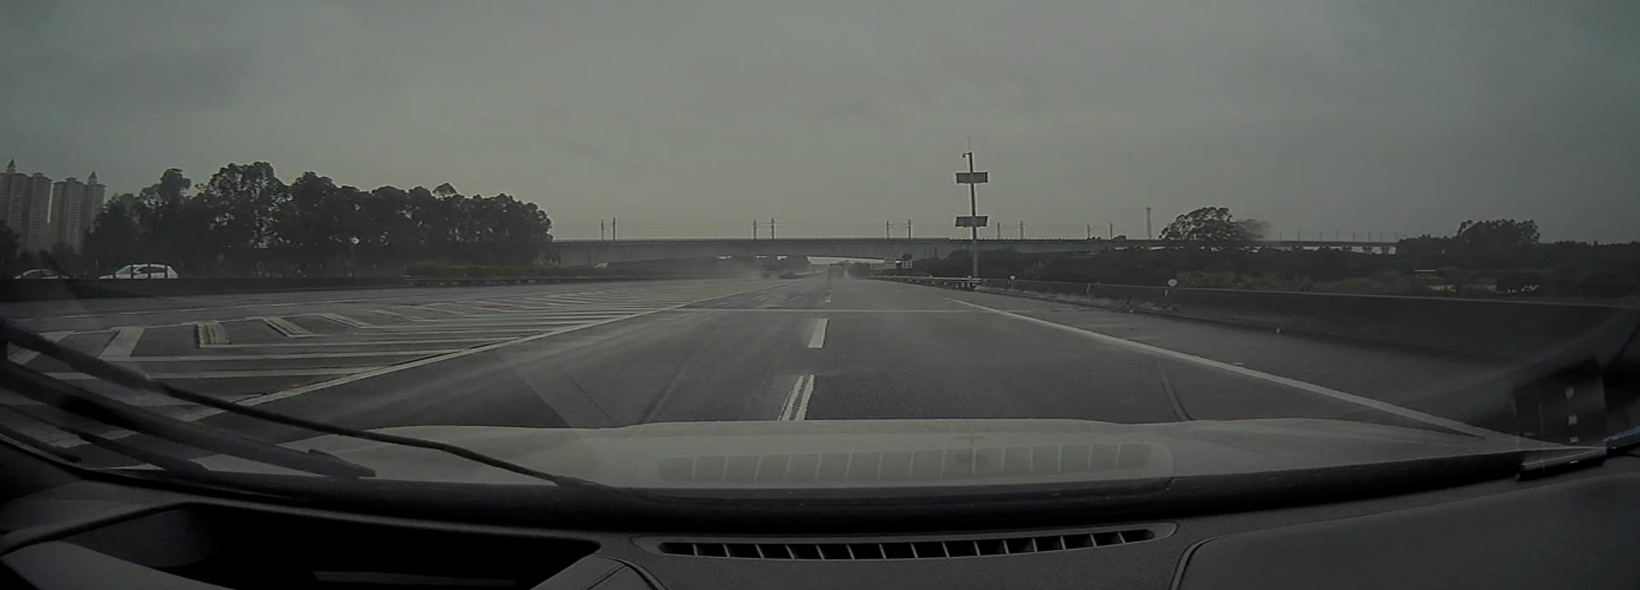
\includegraphics[width=\textwidth]{image/chap03/s4_2427000_原图.jpg}
		\caption{相对清晰的原始场景}
	\end{subfigure}
	\hfill
	\begin{subfigure}[b]{0.48\textwidth}
		\centering
		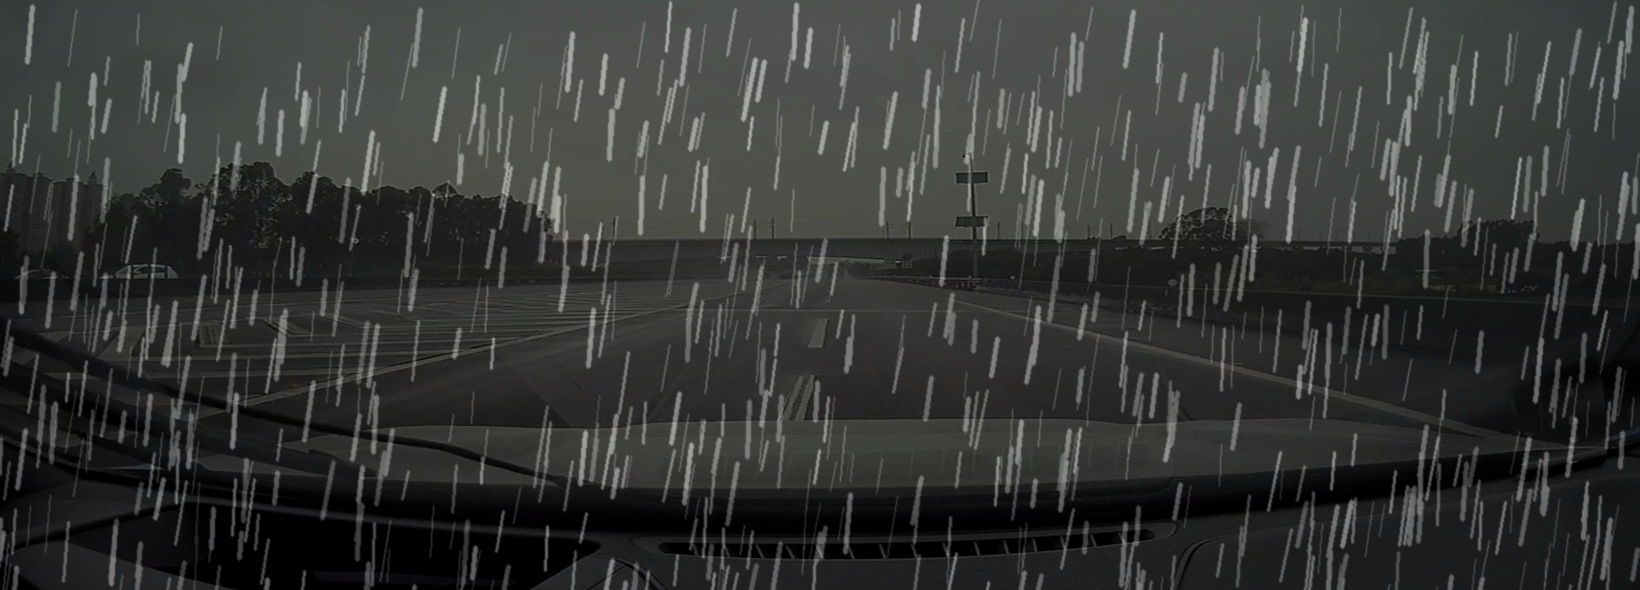
\includegraphics[width=\textwidth]{image/chap03/s4_2427000_中雨.jpg}
		\caption{雨纹增强后的中雨场景}
	\end{subfigure}

	\vspace{0.5em}

	\begin{subfigure}[b]{0.48\textwidth}
		\centering
		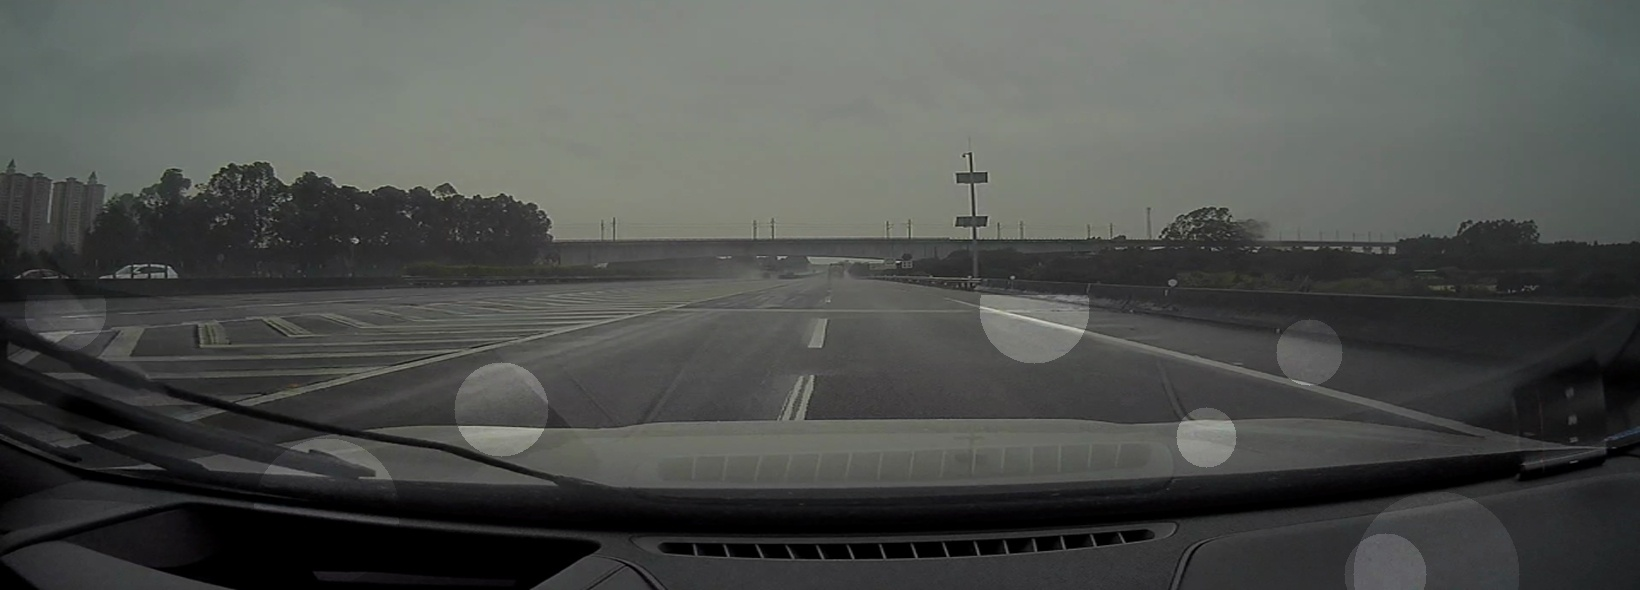
\includegraphics[width=\textwidth]{image/chap03/s4_2427000_重度水膜反射.jpg}
		\caption{水膜反射造成的高亮干扰}
	\end{subfigure}
	\hfill
	\begin{subfigure}[b]{0.48\textwidth}
		\centering
		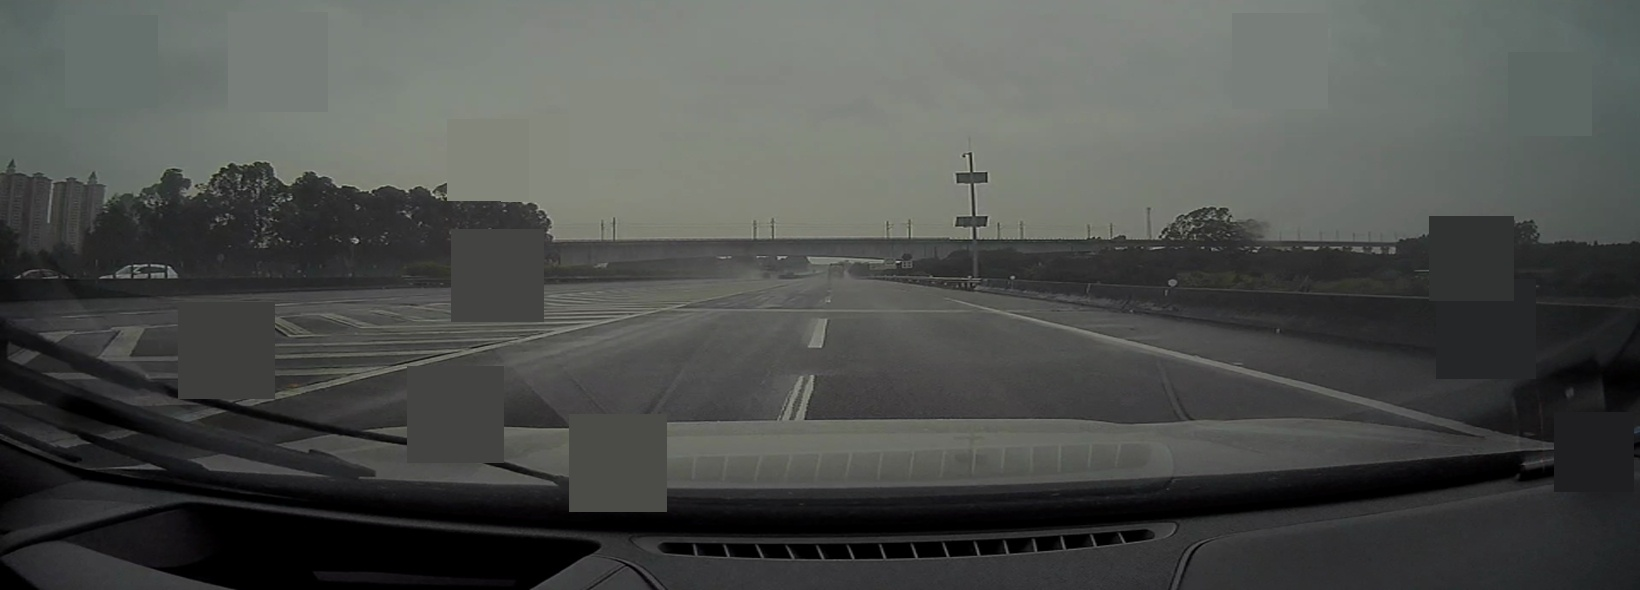
\includegraphics[width=\textwidth]{image/chap03/s4_2427000_重度遮挡.jpg}
		\caption{局部遮挡造成的结构断裂}
	\end{subfigure}
	\caption{雨天车道线检测中几类典型视觉退化现象}
	\label{fig:rain_degradation_theory}
\end{figure}

\subsection{基于物理模型的去雨方法}
经典的图像复原方法基于雨纹的物理成像模型。假设观测图像为清晰背景与雨纹的线性叠加，即 \( I = B + R \)，其中 \( I \) 为雨图，\( B \) 为背景，\( R \) 为雨纹分量。基于稀疏编码、低秩矩阵分解或字典学习的方法通过分离高频雨纹成分实现去雨。然而，该类方法通常假设雨纹具有相似的方向与尺度，对真实雨天中多样化的雨滴形态（大小、形状、运动方向）泛化能力不足。相比之下，深度模型能够更好地学习非线性退化映射，因此逐渐成为单幅图像去雨的主流方向~\cite{fu2017ddn,yang2017jointderain}。

\subsection{基于深度学习的去雨方法}
近年来，卷积神经网络被广泛用于单幅图像去雨任务。Fu等人提出深度细节网络，通过残差映射学习恢复高频细节；Yang等人进一步联合雨纹检测与背景恢复，以提升强降雨场景下的去雨效果；Li等人提出的多阶段上下文聚合网络则强化了不同透明度与方向雨纹的分离能力~\cite{fu2017ddn,yang2017jointderain,li2018rescan}。Zhang等人提出基于多流密集网络的密度感知去雨方法，通过估计雨密度图实现自适应去雨；Porav等人则从物理启发的图像合成角度，利用生成对抗网络（GAN）生成逼真的雨纹，从而训练去雨模型~\cite{zhang2018,porav2019}。这类方法能够有效恢复被雨滴遮挡的图像细节，但网络参数量大、推理耗时长，难以直接嵌入实时ADAS系统。

\subsection{对比度增强与频域滤波方法}
对于雨天车道线检测，车道线与路面之间的低对比度是核心挑战之一。直方图均衡化（HE）、自适应直方图均衡化（CLAHE）以及伽马校正等对比度增强方法可有效拉伸像素灰度分布，提升车道线的视觉显著性，其中CLAHE因对局部区域进行限幅均衡而更适合处理非均匀照明场景~\cite{zuiderveld1994clahe}。此外，频域滤波方法（如小波变换、Gabor滤波）能够分离不同频率成分：雨滴和雨纹对应高频噪声，而车道线的边缘也属于高频信号，但具有特定的方向性和连续性。通过设计方向性滤波器组（如基于车道线方向的Gabor滤波器），可抑制各向同性的雨滴噪声，同时增强具有特定方向的车道线边缘特征~\cite{dunn1995gabor}。该类方法计算开销较小，适合作为轻量级预处理模块与深度学习模型协同工作。

\subsection{图像增强与检测的协同策略}
现有研究多将图像增强作为独立前处理步骤与检测模块串联，二者在特征层面的协同仍相对有限。相比之下，将可微增强模块嵌入网络前端，或在特征提取阶段引入注意力机制，有助于实现更贴近检测目标的联合优化。已有研究表明，自蒸馏、跨层细化和条件卷积等机制，能够在较小额外开销下提升车道线结构表达能力~\cite{hou2019sad,liu2021,zheng2022clrnet}。因此，围绕频域处理与注意力机制的轻量化融合，具有进一步研究的价值。

\section{深度学习轻量化与部署技术}
\label{sec:deep_learning_lightweight}
ADAS车载平台通常具有有限的计算资源与严格的实时性要求（一般要求检测帧率不低于30 FPS）。因此，将深度学习模型部署于边缘端需要进行系统的轻量化设计与推理加速。

\subsection{模型轻量化方法}
\begin{enumerate}[label=(\arabic*)]
	\item \textbf{模型剪枝} \\
	通过移除网络中不重要的权重或神经元，减少模型参数量。结构化剪枝（如通道剪枝）能够直接减少特征图维度，从而加速推理，对硬件友好。经典研究表明，剪枝后再训练可在较小精度损失下显著压缩网络参数规模~\cite{han2015pruning}。
	
	\item \textbf{权重量化} \\
	将浮点型权重和激活值转换为低比特整数表示（如INT8）。量化后模型体积可压缩至原来的1/4，同时利用整数运算加速推理。训练后量化（Post-Training Quantization, PTQ）和量化感知训练（Quantization-Aware Training, QAT）是两种主流策略，后者通常能获得更高的精度保持。Jacob等人的研究系统论证了整数算术推理在移动端的有效性，是当前INT8部署的重要理论基础~\cite{jacob2018quantization}。
	
	\item \textbf{知识蒸馏} \\
	利用大型教师模型指导小型学生模型训练，使轻量模型逼近大模型的性能上限。该方法适用于在保持检测精度的同时压缩模型规模，其基础思想来源于知识蒸馏框架，而在车道线检测中又进一步演化出自蒸馏等轻量化策略~\cite{hinton2015distilling,hou2019sad}。
	
	\item \textbf{高效网络结构设计} \\
	如MobileNet系列中的深度可分离卷积、ShuffleNet中的通道重排、以及轻量级检测头设计~\cite{howard2017mobilenets,sandler2018mobilenetv2,zhang2018shufflenet}。本课题采用的基线模型CLRNet本身已具备较高的效率，但针对雨天场景增加抗干扰模块后仍需进行轻量化优化。考虑到大量车道线检测模型仍以ResNet-18为主干网络，残差结构在精度与部署成熟度上的平衡也具有现实工程价值~\cite{he2016resnet}。
\end{enumerate}

\subsection{边缘端推理加速技术}
\begin{enumerate}[label=(\arabic*)]
	\item \textbf{ONNX模型转换} \\
	ONNX（Open Neural Network Exchange）是一种开放的模型表示格式，支持不同深度学习框架之间的模型互操作。将训练得到的模型导出为ONNX格式后，可进一步导入针对目标硬件优化的推理引擎，以减少运行时框架开销。
	
	\item \textbf{推理引擎优化} \\
	面向GPU的高性能推理引擎通常提供层融合、精度校准、动态张量内存复用等优化手段。具体流程包括：
	\begin{itemize}
		\item \textbf{层融合}：将卷积、批量归一化、激活函数等连续操作融合为单一CUDA内核，减少内存读写与内核启动开销。
		\item \textbf{精度校准}：支持FP32、FP16及INT8推理。INT8推理需提供校准数据集进行激活值分布统计，以最小化量化误差。
		\item \textbf{动态形状支持}：允许模型在推理时接受不同分辨率的输入，增强部署灵活性。
	\end{itemize}
	
	\item \textbf{NVIDIA Orin平台特性} \\
	NVIDIA Orin系统级芯片集成了高达2048个CUDA核心和64个Tensor核心，算力可达200 TOPS（INT8）。其内置的深度学习加速器（DLA）可作为辅助推理引擎，适用于同时运行多个模型任务的场景。本课题将在Orin平台上完成模型转换、TensorRT加速与实时性测试，验证算法在边缘端部署的可行性。
\end{enumerate}

\subsection{精度与速度的权衡策略}
在实际部署中，检测精度、推理速度与功耗之间需要进行权衡。本课题将 FP16 推理作为优先考虑的工程方案，同时保留对 INT8 量化适用性的进一步评估空间。混合精度训练与半精度推理相关研究表明，在合理控制数值范围和累积误差的前提下，半精度通常能够在尽量保持模型性能的同时降低显存占用与计算时延~\cite{micikevicius2018mixedprecision}。因此，后续部署验证将重点关注模型在车载边缘平台上能否兼顾基本检测稳定性与较优时延表现。

\section{本章小结}
\label{sec:summary_2}
本章对本文后续研究所涉及的核心理论与关键技术进行了梳理。从传统图像处理方法与深度学习方法两个角度，概述了车道线检测技术的发展情况，并分析了 CLRNet 作为基线模型的特点及其在雨天场景下面临的局限。结合雨滴、反射和遮挡等典型退化现象，进一步总结了恶劣天气图像增强技术的发展脉络，说明轻量级特征增强与检测协同具有现实可行性。最后，围绕模型轻量化与边缘端部署技术，介绍了剪枝、量化、推理图优化以及 NVIDIA Orin 平台相关内容，为后续算法设计与部署验证提供了技术背景。

% TODO：增加引用例子。
